\documentclass[11pt,a4paper]{article}
\usepackage[margin=23mm,headheight=15pt]{geometry}
\usepackage{amsmath,graphicx,booktabs,fancyhdr,lastpage}
\usepackage{listings}\lstset{language=Python,basicstyle=\ttfamily\footnotesize,breaklines=true,columns=fullflexible,keepspaces=true,literate={–}{{-}}1}
\usepackage[hidelinks]{hyperref}
\graphicspath{{../results/}}
\InputIfFileExists{team-local.tex}{}{\newcommand{\TeamNumber}{\phantom{apmcm26300001}}}
\pagestyle{fancy}
\fancyhf{}
\fancyhead[L]{Team \TeamNumber}
\fancyhead[R]{Page \thepage\ of \pageref{LastPage}}
\setlength{\parskip}{5pt}
\setlength{\parindent}{0pt}
\newcommand{\callname}[1]{\textsc{#1}}
\newcommand{\evidence}[2]{\href{https://github.com/feiniao87968492-stack/apmcm-2026-problem-c/blob/41f7153643d6098940507a8682c2bcbb4d64f97f/#1}{#2}}
\newcommand{\coreevidence}[2]{\href{https://github.com/feiniao87968492-stack/apmcm-2026-problem-c/blob/0b74512/#1}{#2}}
\newcommand{\followupevidence}[2]{\href{https://github.com/feiniao87968492-stack/apmcm-2026-problem-c/blob/d21e3e5/#1}{#2}}
\newcommand{\monitoringevidence}[2]{\href{https://github.com/feiniao87968492-stack/apmcm-2026-problem-c/blob/c941a0713ac8305839d7d8a2c258a987df5d9523/#1}{#2}}
\newcommand{\PaperSummary}{We analyze 108 calls and 139 paired playback experiments in four linked models. A grouped acoustic classifier using six shared measurements gives macro F1 of 0.225, compared with 0.207 for the fold-majority model. At a fidelity threshold of 0.50, flat, modulated and two-voice calls have acoustic ranges of 84.7, 144.6 and 169.7 m. Natural calls elicited a response in 90 of 139 playbacks, compared with 18 of 139 controls. The observed paired difference was 51.8 percentage points, with a 95\% paired bootstrap interval of 43.9--60.1 points. The integrated clean effectiveness radii are 87.0 m, 131.7 m and at least 150 m, respectively. Under a modeled 20\% fidelity loss, those distances fall to 46.0, 70.4 and 124.3 m. We report the uncertainty and sensitivity of these operational distances and outline a field design for evaluating noise in foraging areas.}

\newcommand{\AcousticResults}{Peak frequency was the only acoustic measure reaching 5\% in the Holm-adjusted omnibus tests ($p=0.0130$). The significant pairwise difference was flat versus modulated peak frequency ($p=0.0244$). The grouped macro F1 was 0.225 with a recording-group bootstrap range of 0.145--0.286, versus 0.207 for the majority baseline. Adding median-imputed pulse rate gave 0.259. Pulse rate was absent in all flat calls and missing in some modulated and two-voice calls. Availability of F02 alone gave 0.569 because F02 was recorded only for the two-voice category. Held-out permutation scores did not identify a stable positive contribution from a shared feature. We carry the supplied call labels into propagation and behavior modeling. The peak-frequency result motivates retaining a spectral component in the fidelity measure. The weak grouped classifier supports using measured call labels rather than assigning new labels from acoustic features.
\par\begin{center}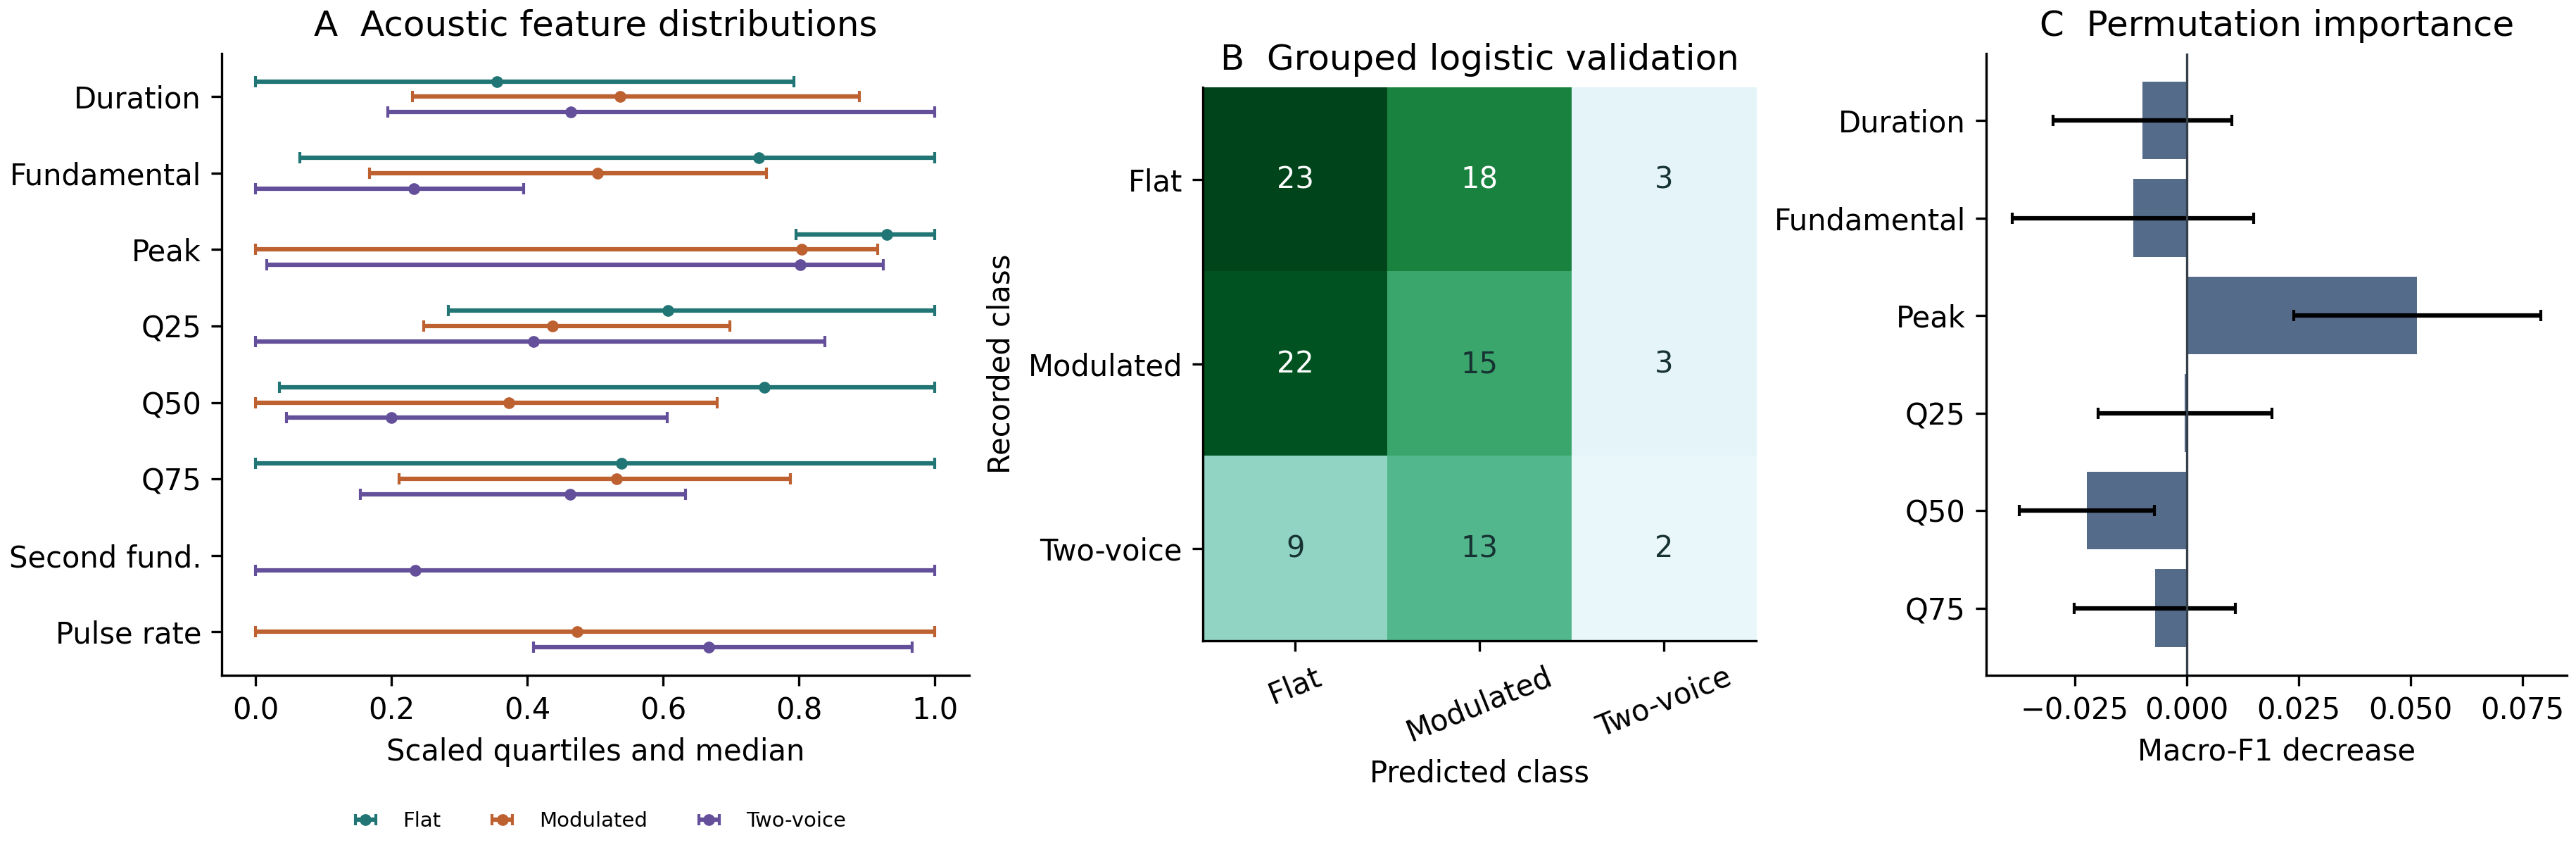
\includegraphics[width=.92\linewidth]{q1_acoustics.png}\\
{\small Figure 1. Acoustic summaries, grouped classification and held-out permutation importance.}\end{center}}

\newcommand{\PropagationResults}{
\begin{center}\small
\begin{tabular}{lrrr}
\toprule
Call & 0.40 & 0.50 & 0.60\\
\midrule
Flat & 113.5 [111.8,115.2] & 84.7 [83.7,85.9] & 62.6 [60.6,64.4]\\
Modulated & 181.7 [180.0,183.9] & 144.6 [142.3,147.1] & 109.2 [106.9,112.0]\\
Two-voice & 203.9 [202.7,205.1] & 169.7 [168.9,170.6] & 141.3 [140.5,142.0]\\
\bottomrule
\end{tabular}\\[3pt]
Table 1. Propagation ranges in metres, with 95\% conditional bootstrap intervals.
\end{center}
Two-voice has the longest estimated range at the three primary thresholds under the tested weights. At 0.70, the equal-weight estimate for two-voice is close to that for modulated calls and their uncertainty intervals overlap. Increasing the envelope weight can reverse their ranking at 0.70. Choice of the similarity criterion therefore matters most for claims about very reliable recognition.
\par\begin{center}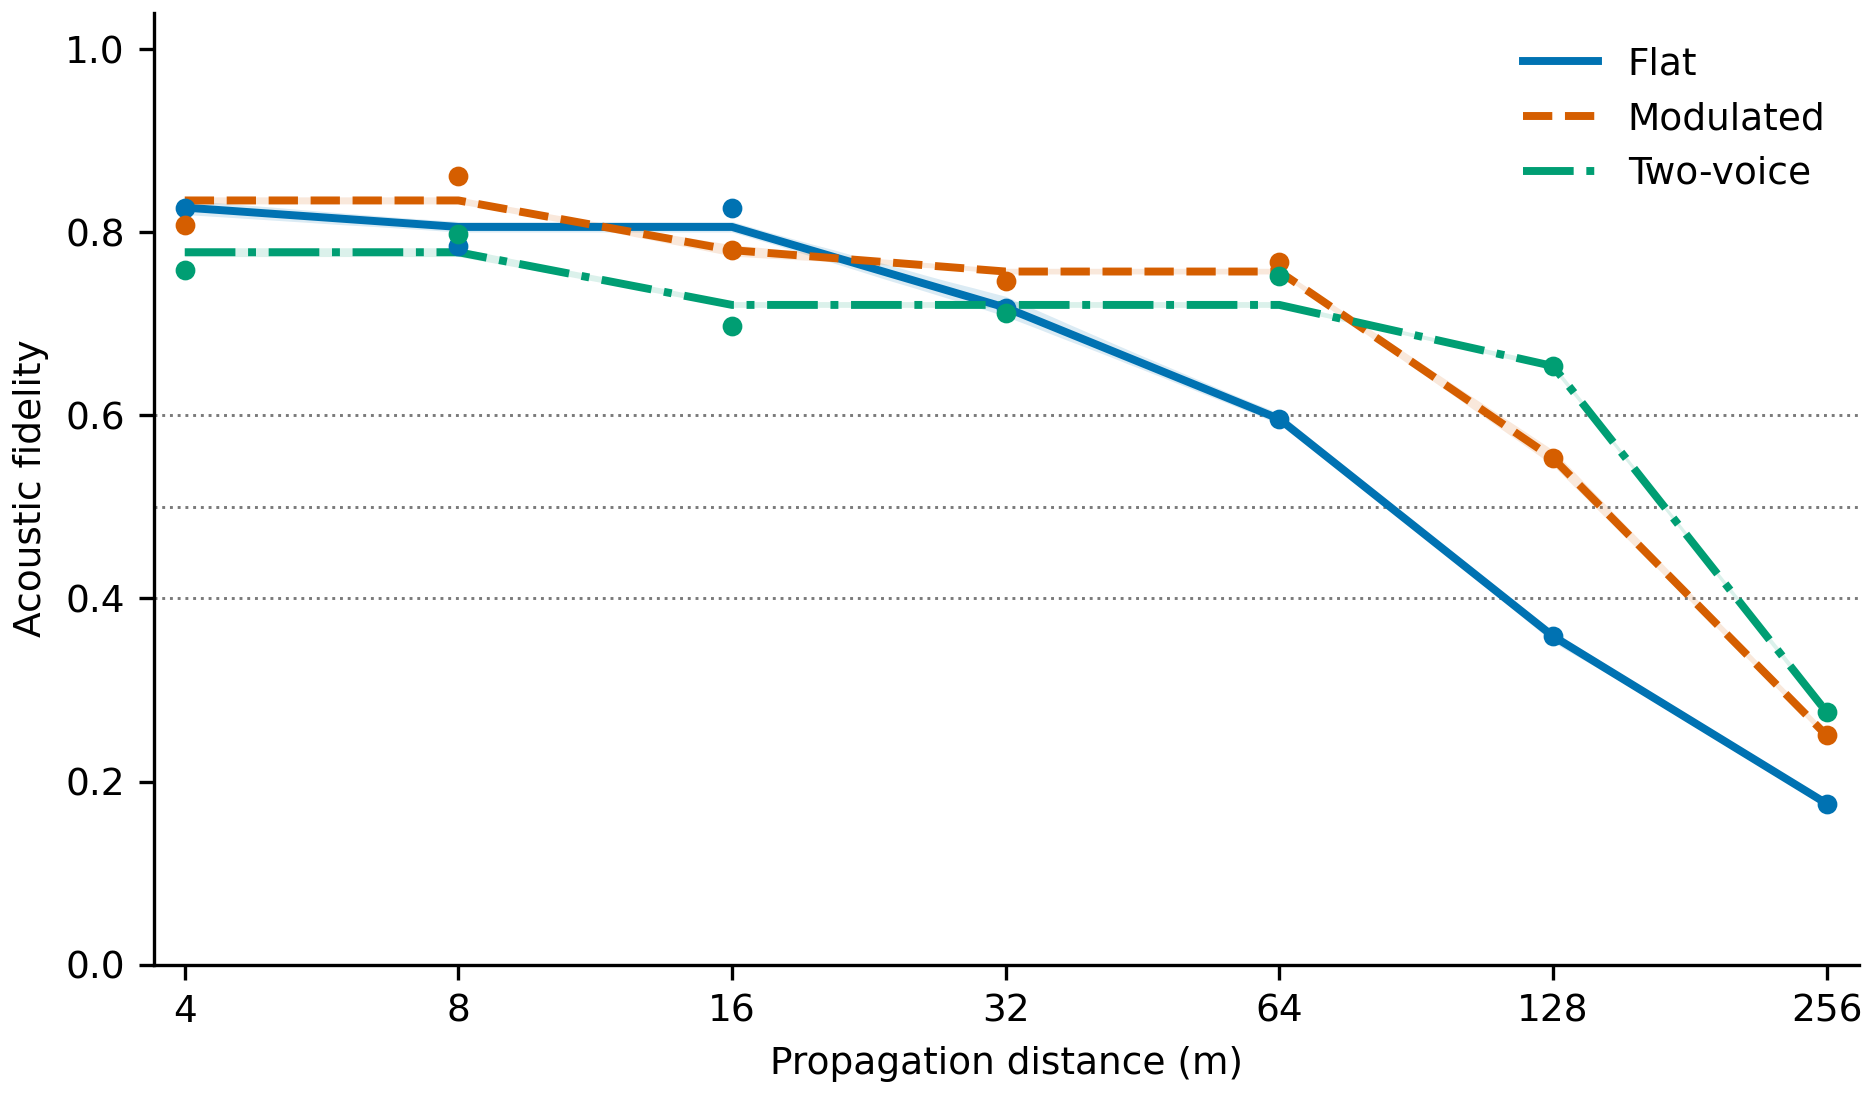
\includegraphics[width=.94\linewidth]{q2_propagation.png}\\{\small Figure 2. Equal-weight fidelity and conditional propagation intervals.}\end{center}}

\newcommand{\BehaviorResults}{
There were 74 pairs with a response only to the natural call, two with a response only to control, 16 with both and 47 with neither. The exact McNemar $p$ value was $7.75\times10^{-20}$ for equality of the observed paired marginal response rates. With grouped validation, the multinomial model had a mean mask log loss of 1.245, versus 1.384 for pooled training frequencies. The corresponding Brier scores for any response were 0.154 and 0.238. At 50 m and eight observed birds, the adjusted natural-call increment for the vocal-only response to flat calls was 0.134, with an interval of 0.043--0.276. The full combination distribution includes joint responses and baseline controls.
\par\begin{center}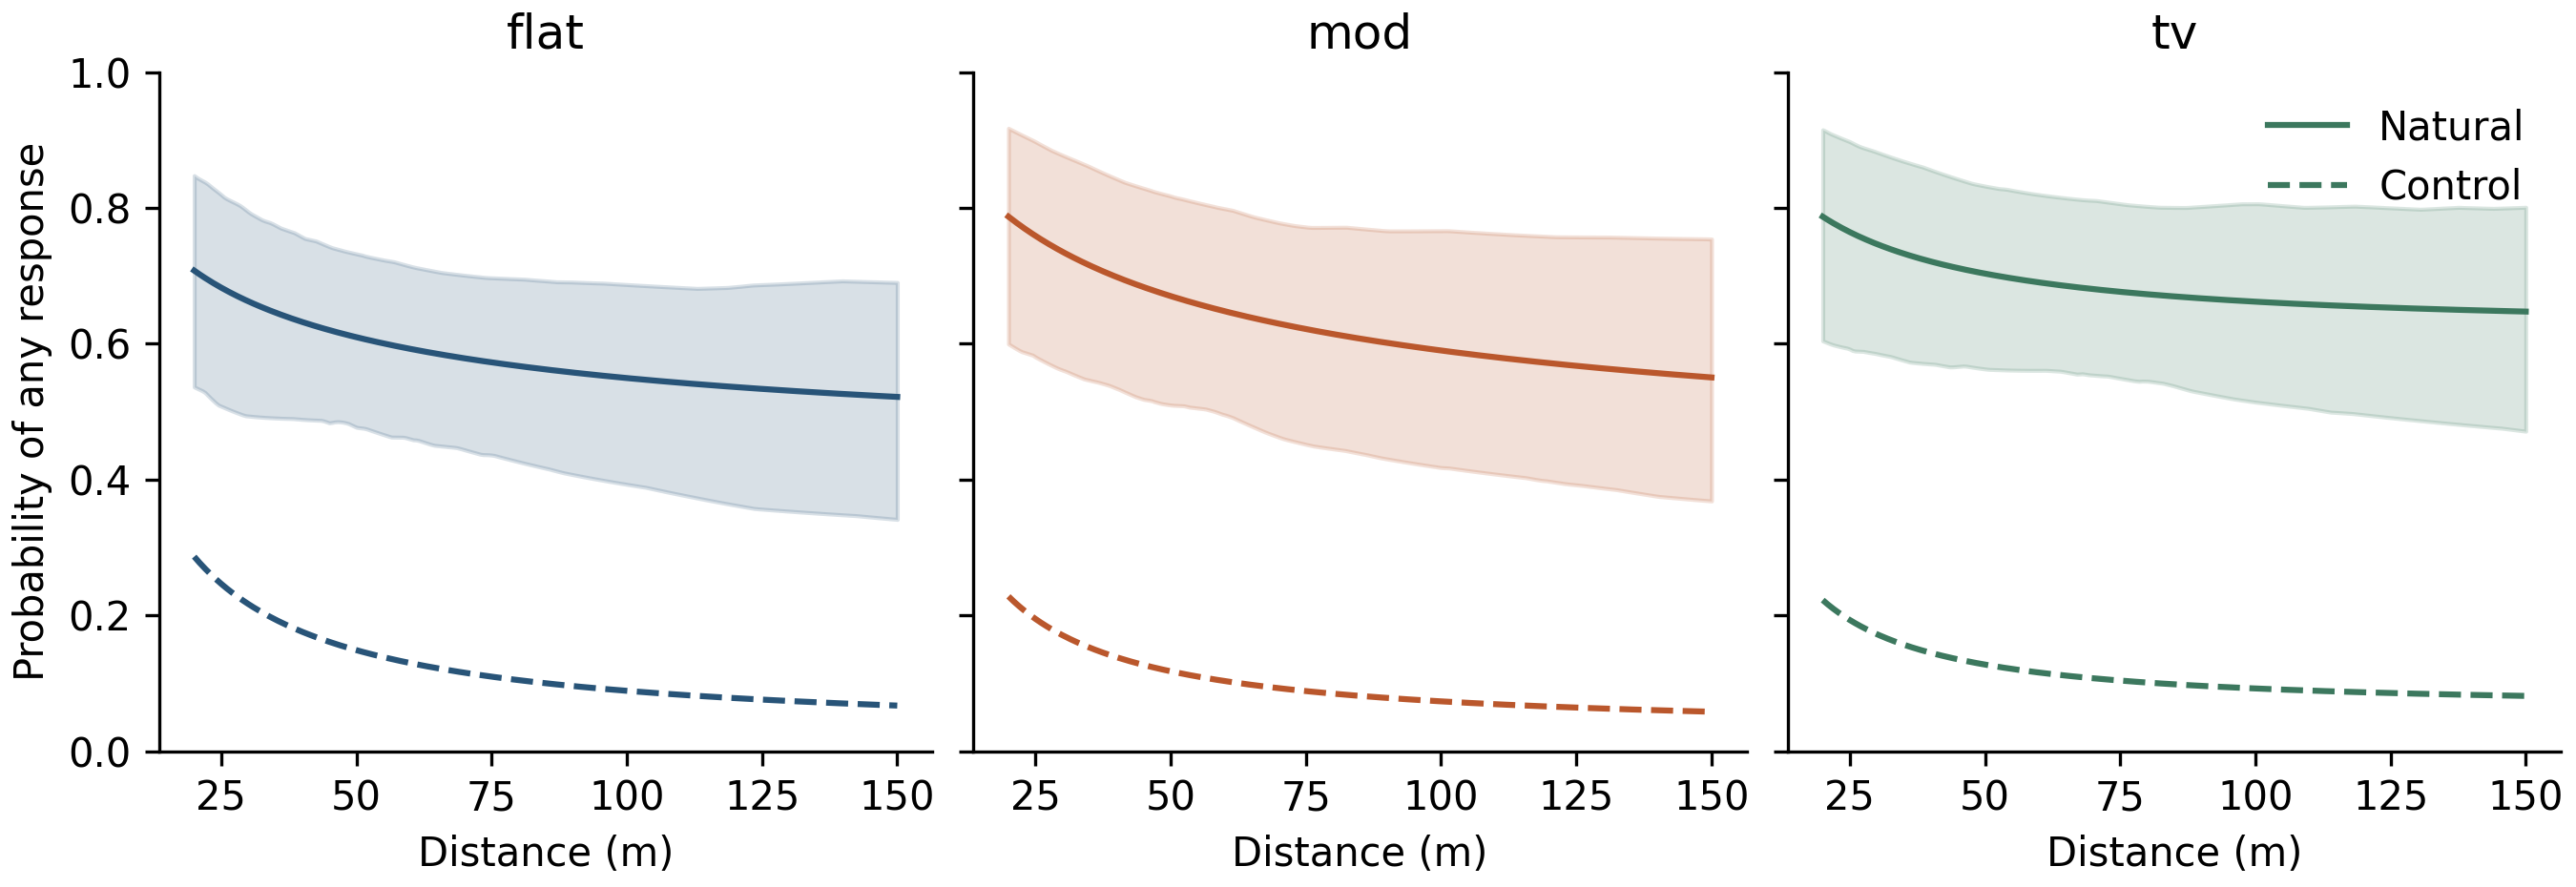
\includegraphics[width=.87\linewidth]{q3_response_curve.png}\\{\small Figure 3. Adjusted any-response probabilities. Shading shows paired bootstrap intervals for natural stimuli.}\end{center}
\begin{center}\small
\begin{tabular}{lrrr}
\toprule
Call & 50 m & 100 m & 150 m\\
\midrule
Flat & 1.79 & 1.88 & 1.94\\
Modulated & 1.81 & 1.91 & 1.96\\
Two-voice & 2.10 & \TVHundred & \TVFar\\
\bottomrule
\end{tabular}\\[3pt]
Table 2. Predicted median onset of head raising in seconds, conditional on head raising, for natural calls and eight birds.
\end{center}
At 150 m, the flat and modulated onset estimates use information pooled from the wider dataset because no observed head-raising onsets occur within 25 m in those call strata. Control stimuli produced no observed approaches, leaving their conditional approach onset unavailable. Tables accompanying the paper contain each behavior's probabilities and latency estimates at all three distances, along with the vocal-count and duration summaries.}

\newcommand{\IntegratedResults}{
\begin{center}\small
\begin{tabular}{lrrr}
\toprule
Call & Clean & 20\% loss & Threshold 0.70\\
\midrule
Flat & 87.0 & 46.0 & 35.2\\
Modulated & 131.7 & 70.4 & 77.6\\
Two-voice & $\ge 150$ & 124.3 & 79.2\\
\bottomrule
\end{tabular}\\[3pt]
Table 3. Integrated radii in metres, using the fixed 50\% clean reference.
\end{center}
The clean flat radius has a conditional bootstrap range of 64.8--121.0 m. The modulated and two-voice intervals reach the upper study bound. At the same relative criterion, the behavior-only model reaches the support limit for every call. Integrating the acoustic component provides an in-range crossing for flat and modulated calls. The acoustic-only radius for flat calls is 117.3 m and the integrated estimate is 87.0 m. At 100 m, the modeled 20\% loss changes response probabilities from 0.549, 0.590 and 0.662 to 0.457, 0.487 and 0.548 for flat, modulated and two-voice calls, respectively. If half of an eight-bird responding group participates, those three altered probabilities imply mean counts of about 1.83, 1.95 and 2.19. The rank in the clean point estimates is stable across the two alternative acoustic weights, with the two-voice result bounded by support.
\par\begin{center}\begin{minipage}{.94\linewidth}\centering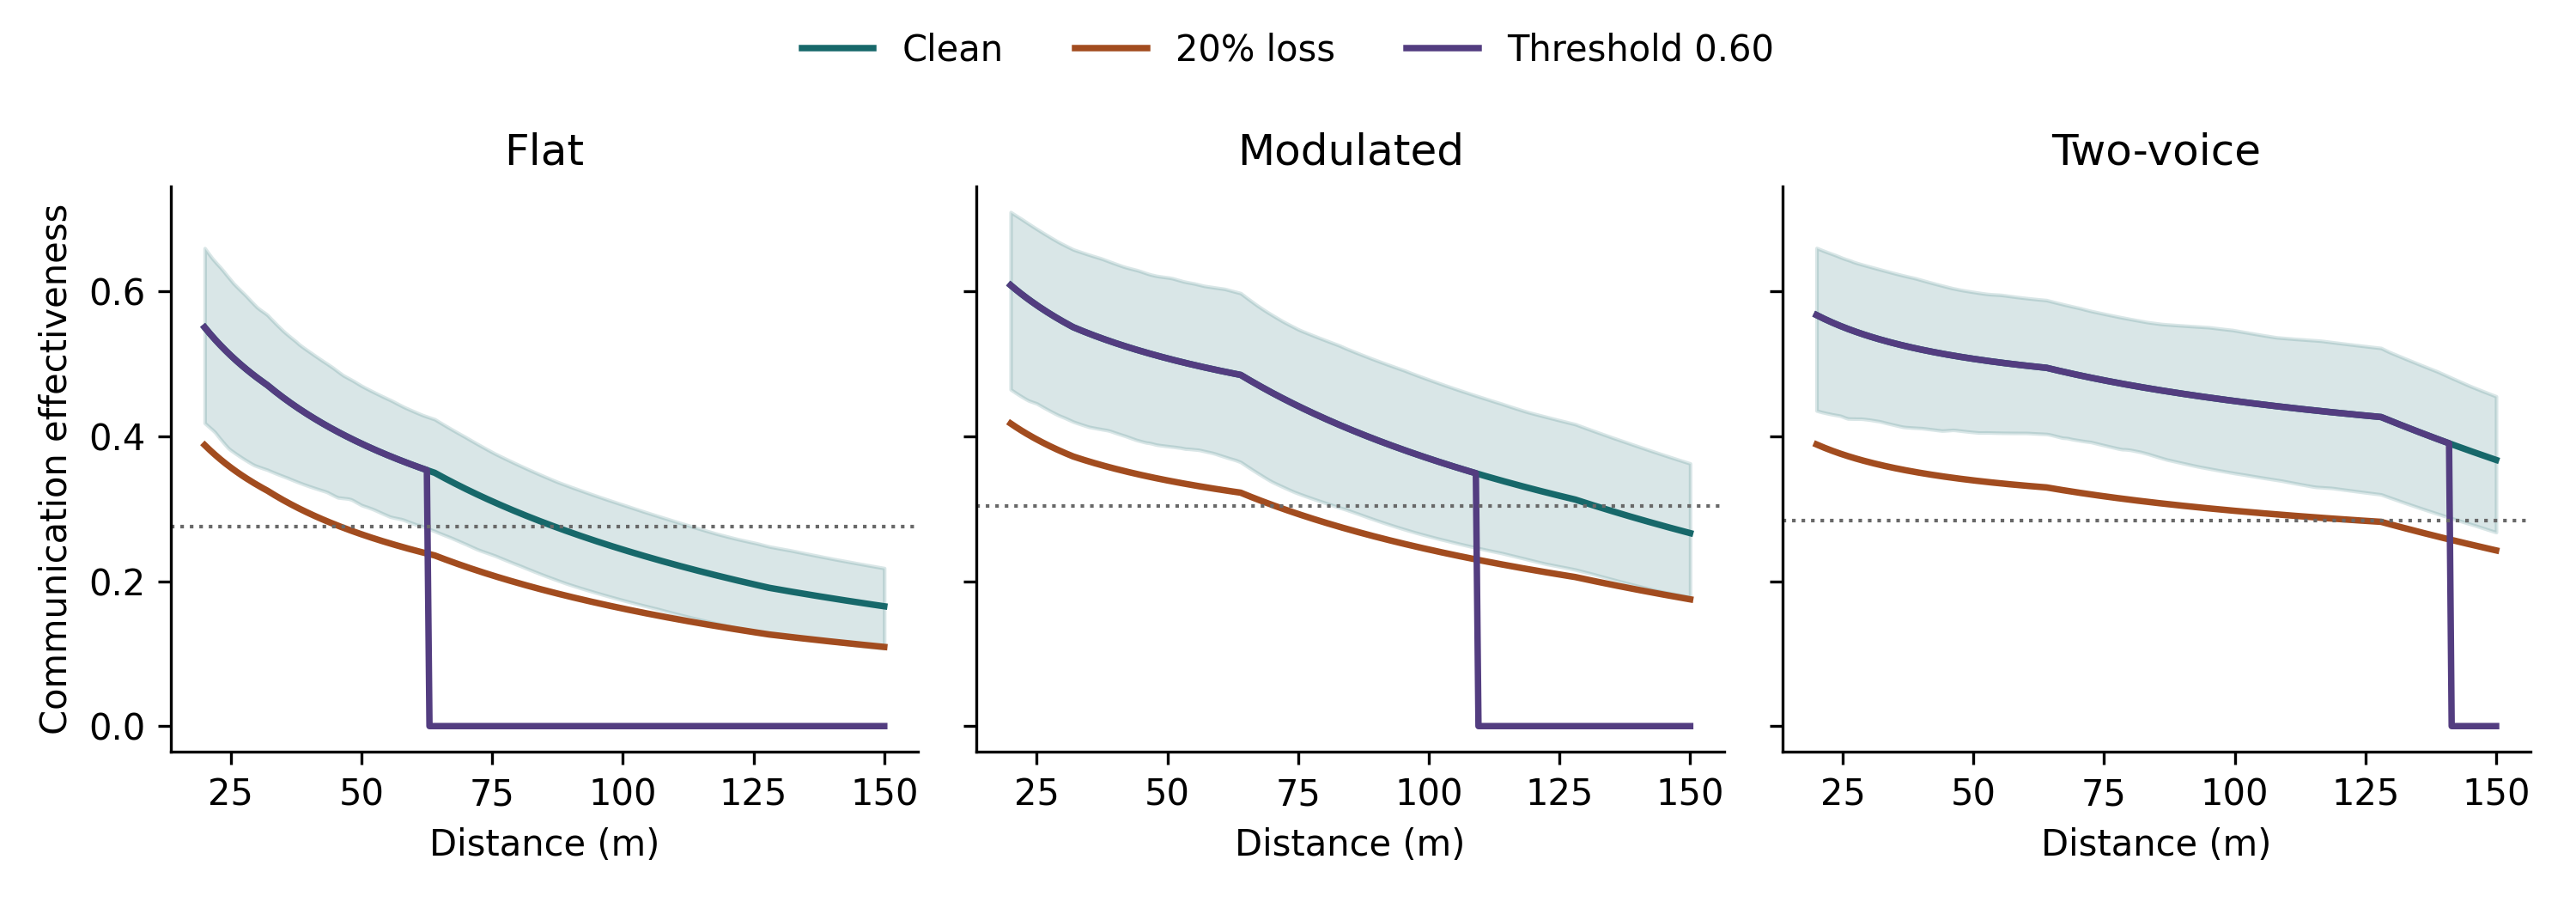
\includegraphics[width=\linewidth]{q4_scenarios.png}\\{\small Figure 4. Integrated effectiveness by distance. Dotted lines mark the fixed clean reference and shading shows the clean conditional interval.}\end{minipage}\end{center}}

\newcommand{\TVHundred}{2.20}
\newcommand{\TVFar}{2.26}




\begin{document}

\begin{center}
{\small 2026 Asia and Pacific Mathematical Contest in Modeling}\\[1em]
{\large Problem C \quad \TeamNumber}\\[2em]
{\LARGE How far can African penguin calls support communication at sea?}
\end{center}
\vspace{1em}
\section*{Summary}
\PaperSummary

\textbf{Keywords}\quad African penguin, playback experiment, acoustic fidelity, grouped validation, communication radius

\clearpage
\tableofcontents
\clearpage

\section{Question and evidence}
African penguins use several call types at sea. A useful comparison needs to account for differences in the recorded call features, the loss of signal fidelity over distance, and the behaviors observed after playback. We analyze the acoustic recordings, propagation trials and paired playback data supplied with Problem C \cite{problem,archive}. We use acoustic recordings to characterize the calls, propagation tables to estimate signal retention, and paired stimuli to distinguish behavioral responses to natural calls from background responses to control sounds.

We treat the playback group as the observational unit for behavior. A positive group outcome means at least one of the scored behaviors was observed. The integrated radius is an operational measure defined on the distance range supported by both data sources. Its interpretation depends on the chosen reference level and experimental context.

\section{Acoustic characteristics and classification}
The recording date and location define groups for held-out validation. The baseline feature set contains duration, first fundamental frequency, peak frequency, and three spectral quartiles. The adopted model uses six physical coordinates derived from those measurements. The second fundamental contributes to the descriptive analysis of two-voice calls. Because its availability is associated with the call type in the supplied recordings, we analyze that field separately from the main classifier.

We use rank tests with Holm correction to describe acoustic differences. Nested date-location folds choose settings from training recordings. We score pooled held-out macro F1, class recall, log loss and Brier, with a paired recording-group bootstrap for F1. A replacement must improve F1 at the paired lower limit, preserve two-voice recall and improve both proper scores over training prevalence.

\AcousticResults

\section{Propagation, signal fidelity and recognition criteria}
Let $\bar r_{cm}(d)$ be the available-case mean correlation with the one-metre reference for call type $c$, representation $m$ and distance $d$. The representations are the spectrogram, amplitude spectrum, and amplitude envelope. Propagation was measured at Brandvlei Dam in December 2021 under calm conditions \cite{fieldstudy}. For each call type, three examples contributed up to $10\times10$ comparisons of reference and distant repetitions per example. We clip their equal-weight mean to $[0,1]$ at the seven measured distances. For a positive signal gain in $Y=a(d)X+\epsilon$ with independent additive noise,
\[
\operatorname{Corr}(X,Y)=
\left[1+\frac{\operatorname{Var}(\epsilon)}{a(d)^2\operatorname{Var}(X)}\right]^{-1/2}.
\]
We fit a call-specific ceiling, reference scale and effective spreading exponent. The adopted fidelity curve is
\[
 F_c(d)=A_c\bigl[1+(d/D_c)^{g_c}10^{\alpha_c(d-1)/10}\bigr]^{-1/2}.
\]
The spreading component uses the fitted effective exponent $g_c$. The atmospheric component uses $\alpha_c$ in dB/m from ISO 9613-1 \cite{iso9613}. Partial pooling shrinks the three log exponents toward their mean. Weather inputs are fixed at 20\,$^\circ$C, 70\% relative humidity and 101.325 kPa. We compare type-specific medians of peak frequency and spectral Q50. These correlations omit calibrated received levels and a linkage between waveforms and propagation examples, so the absorption coefficient is supplied by assumption. Model selection uses both interior holdouts and forward fits using strictly shorter distances. We compare equal-weight cell RMSEs and 300 paired wide-row resamples.

\PropagationResults

\clearpage
\section{Paired playback responses}
In the \href{https://doi.org/10.12688/openreseurope.24618.1}{original field protocol}, each observed penguin group received one natural call playback and one sea-wave control playback in randomized order. The researchers randomly drew natural tracks without replacement within each behavioral context. Data02 records the group-level response to each stimulus and links the two observations by experiment identifier. Playback distances differed within 90 of the 139 pairs. The raw within-pair comparison describes the sampled stimuli. The adjusted prediction model retains the measured covariates and evaluates both stimulus conditions at identical covariate values. Natural call type is assigned to both trials. We also stratify paired response differences by relative playback distance and use date-block bootstrap intervals.

An eight-state mask records the combination of the three scored behaviors. The full multinomial uses stimulus, call type and their interaction, context, log distance and log group size. The strict comparison holds out each of 12 dates and purges any additional pair sharing a held natural track. Alternatives include stimulus frequencies, a structured pairwise model, a shrinkage hurdle, a rank-one tilt and a training-only nested pool. We compare mask log loss and any-response Brier with paired date intervals.

We analyze observable event time over the field protocol's 60 s window, for the first flagged event and each individual behavior. Cumulative time bins include zero, 5, 15, 30 and 60 s, with a separate administrative censoring cell. We compare stimulus frequencies, a regularized discrete hazard, a finite-window occurrence model and a Weibull accelerated failure-time model on the same folds. We score censored log loss and integrated Brier, with conditional MAE as a secondary comparison. Distance-specific predictions use eight birds, average over observed contexts and display local trial support. The time estimand ends at 60 s.

Head-raising duration is the recorded span between the first bird starting and the last bird stopping within the 60 s observation window. We compare paired seconds per trial, including zeros, and mean seconds among responders. A two-part model predicts expected seconds by multiplying the probability of a positive span by its conditional mean. We compare each part with and without natural call-type terms, scoring expected seconds on the same held dates.

\BehaviorResults

\clearpage
\section{Integrated communication and conservation}
Let $p_c(d)$ be the natural-stimulus any-response probability at median group size, averaged over the observed contexts. We define gross communication effectiveness as
\[
E_c(d)=F_c(d)p_c(d).
\]
The production Q4 path uses the selected propagation curve. To attribute changes, we cross the selected and archived acoustic and behavioral components at the same distances and apply a common gross threshold. It is half the equal-call clean mean from the archived isotonic and multinomial fits at 20 m. The product radius is the sustained downward crossing of that threshold. Under hypothetical 20\% coupled loss, fidelity decreases by 20\% and the natural probability decreases by 20\% of positive natural-minus-control response excess.

A second rule requires both fidelity and the cumulative natural probability by 30 s to attain 0.50 at each prefix node from 20 m. We also evaluate 15 s. These thresholds describe a planning scenario. The common evaluation grid ends at 150 m, and sparse local playback support limits interpretation near that boundary.

\IntegratedResults

Pilot quiet windows during mapped foraging activity or reroute vessels around those areas when navigation permits. Compare usual operations with the pilot under comparable sea states and group contexts. Measure calibrated noise levels and spectra at receiver positions, and compare recorded responses to paired natural and control playbacks with counterbalanced presentation order. Sample across the 80--130 m span where the two-voice scenario endpoints differ and near 150 m to check the far-distance extrapolation. Use the modeled distances as conditional planning inputs, with any operating buffer subject to local noise and behavioral calibration. Record acquisition identifiers, contexts and playback order. The earlier monitoring, noise, carryover and trial-design comparisons remain available in the supporting analyses. \coreevidence{README.md}{Supporting analyses and reproduction}.

\section{Limitations and reproducibility}
Sparse responses limit precision for behavior combinations and onset times. The integrated index combines separate propagation and playback experiments. Its noise scenarios depend on the stated assumptions. The public recordings include one waveform example per call type. An earlier sea-surface archive provides call codes and behavioral context \cite{earliersurface}. An independent acoustic validation needs waveform or spectral records linked to all three labels and acquisition groups. Data02 provides no verified stimulus order, so presentation-order and carryover effects are unestimated. The \href{https://github.com/feiniao87968492-stack/apmcm-2026-problem-c/blob/aaaff78e98df91bc998fa1359171050e7b1967a8/docs/data-audit.md\#playback-design-and-order-recoverability}{versioned playback audit} documents the available design fields. The repository provides code and results. The specification records resampling counts and seeds for each analysis.

\begin{thebibliography}{9}
\bibitem{problem} APMCM Organizing Committee. 2026 APMCM Problem C, \emph{Acoustic Communication and Playback Responses of African Penguins at Sea}. Contest statement and attachments, 2026.
\bibitem{archive} \emph{African penguin acoustic and playback study, associated data and supplementary material}. Zenodo record 21376649, \url{https://zenodo.org/records/21376649}, accessed November 26, 2026.
\bibitem{fieldstudy} Thiebault, A., et al. Contact and recruit: the importance of acoustic communication in the foraging strategy of a flightless seabird. \emph{Open Research Europe}, 2026. \url{https://doi.org/10.12688/openreseurope.24618.1}.
\bibitem{earliersurface} McInnes, A. M., et al. Social context and prey composition are associated with calling behaviour in a diving seabird. \emph{Ibis}, 162, 1047--1059, 2020. \url{https://doi.org/10.1111/ibi.12806}. Data at \url{https://doi.org/10.6084/m9.figshare.7212173.v2}.
\bibitem{boatnoise} Thiebault, A., et al. African penguins' behaviour is affected by motor boat airborne noise: an experimental study on wild penguins. \emph{Science of the Total Environment}, 1056, 182372, 2026. \url{https://doi.org/10.1016/j.scitotenv.2026.182372}.
\bibitem{iso9613} International Organization for Standardization. ISO 9613-1:1993, \emph{Acoustics: Attenuation of sound during propagation outdoors. Part 1: Calculation of the absorption of sound by the atmosphere}.
\bibitem{era5} Copernicus Climate Change Service. ERA5 hourly data on single levels, accessed through Open-Meteo on November 26, 2026. \url{https://doi.org/10.24381/cds.adbb2d47}.
\bibitem{waverys} Copernicus Marine Service. Global Ocean Waves Reanalysis (WAVERYS), product GLOBAL\_MULTIYEAR\_WAV\_001\_032.
\end{thebibliography}
\clearpage
\appendix
\section{Archived conditional-onset sensitivity}
Cells show predicted event probability and conditional median onset in seconds.
The symbol -- marks an unavailable onset estimate. A dagger marks sparse local support.
\begin{center}\begin{minipage}{.94\linewidth}\centering\small
\textbf{Head raising}\\[3pt]
\begin{tabular}{llrrr}\toprule
Stimulus & Assigned call & 50 m & 100 m & 150 m\\\midrule
Natural & Flat & 0.457 / 1.79 & 0.354 / 1.88 & 0.300 / 1.94$^\dagger$\\
Natural & Modulated & 0.482 / 1.81 & 0.365 / 1.91$^\dagger$ & 0.305 / 1.96$^\dagger$\\
Natural & Two-voice & 0.371 / 2.10 & 0.261 / 2.20 & 0.208 / 2.26$^\dagger$\\
Control & Flat & 0.137 / 1.23$^\dagger$ & 0.075 / 1.31$^\dagger$ & 0.052 / 1.35$^\dagger$\\
Control & Modulated & 0.101 / 1.47$^\dagger$ & 0.053 / 1.55$^\dagger$ & 0.036 / 1.60$^\dagger$\\
Control & Two-voice & 0.088 / 1.41$^\dagger$ & 0.046 / 1.49$^\dagger$ & 0.032 / 1.54$^\dagger$\\
\bottomrule\end{tabular}
\end{minipage}\end{center}
\begin{center}\begin{minipage}{.94\linewidth}\centering\small
\textbf{Vocalizing}\\[3pt]
\begin{tabular}{llrrr}\toprule
Stimulus & Assigned call & 50 m & 100 m & 150 m\\\midrule
Natural & Flat & 0.531 / 3.17 & 0.507 / 3.63 & 0.492 / 3.92$^\dagger$\\
Natural & Modulated & 0.493 / 2.67 & 0.489 / 3.08$^\dagger$ & 0.479 / 3.33$^\dagger$\\
Natural & Two-voice & 0.575 / 3.71 & 0.596 / 4.23 & 0.604 / 4.56$^\dagger$\\
Control & Flat & 0.019 / -- & 0.019 / -- & 0.020 / --\\
Control & Modulated & 0.020 / 4.68$^\dagger$ & 0.023 / 5.30$^\dagger$ & 0.024 / 5.70$^\dagger$\\
Control & Two-voice & 0.043 / 5.72$^\dagger$ & 0.048 / 6.46$^\dagger$ & 0.052 / 6.93$^\dagger$\\
\bottomrule\end{tabular}
\end{minipage}\end{center}
\begin{center}\begin{minipage}{.94\linewidth}\centering\small
\textbf{Approaching}\\[3pt]
\begin{tabular}{llrrr}\toprule
Stimulus & Assigned call & 50 m & 100 m & 150 m\\\midrule
Natural & Flat & 0.079 / 9.11$^\dagger$ & 0.055 / 11.52$^\dagger$ & 0.045 / 13.21$^\dagger$\\
Natural & Modulated & 0.245 / 8.06 & 0.201 / 10.22$^\dagger$ & 0.178 / 11.73$^\dagger$\\
Natural & Two-voice & 0.199 / 7.99 & 0.139 / 10.16$^\dagger$ & 0.112 / 11.67$^\dagger$\\
Control & Flat & 0.003 / -- & 0.002 / -- & 0.002 / --\\
Control & Modulated & 0.003 / -- & 0.002 / -- & 0.002 / --\\
Control & Two-voice & 0.003 / -- & 0.002 / -- & 0.002 / --\\
\bottomrule\end{tabular}
\end{minipage}\end{center}


\section{Archived behavior combinations}
\begin{center}
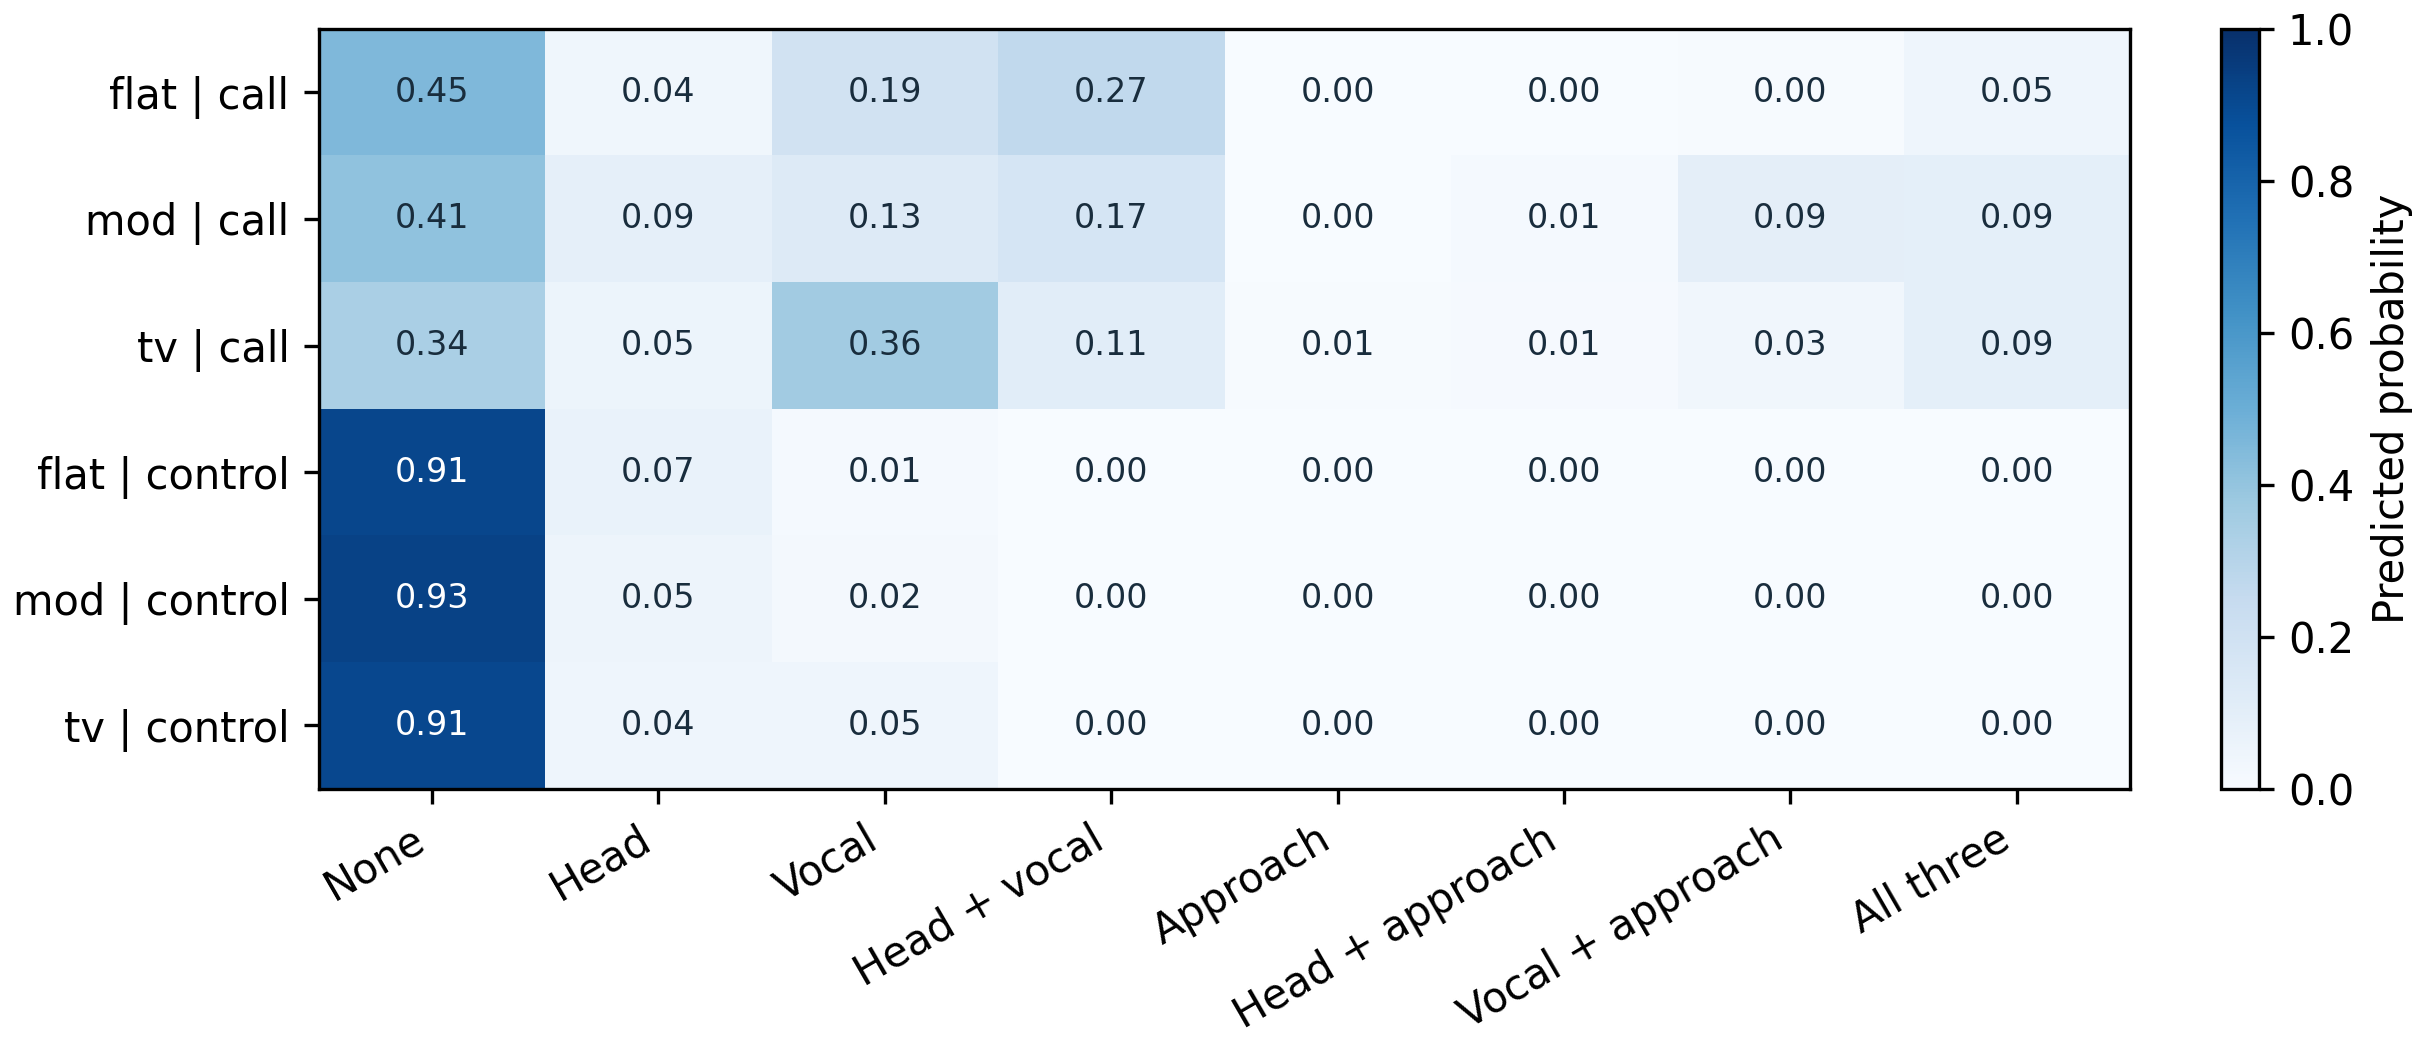
\includegraphics[width=.96\linewidth]{q3_behavior_masks.png}\\
{\small Figure B1. Archived multinomial behavior combinations for natural and control stimuli at 100 m and eight birds, averaged over empirical context frequencies.}
\end{center}

\section{Call-specific disturbance scenarios}
\begin{center}\begin{minipage}{.94\linewidth}\centering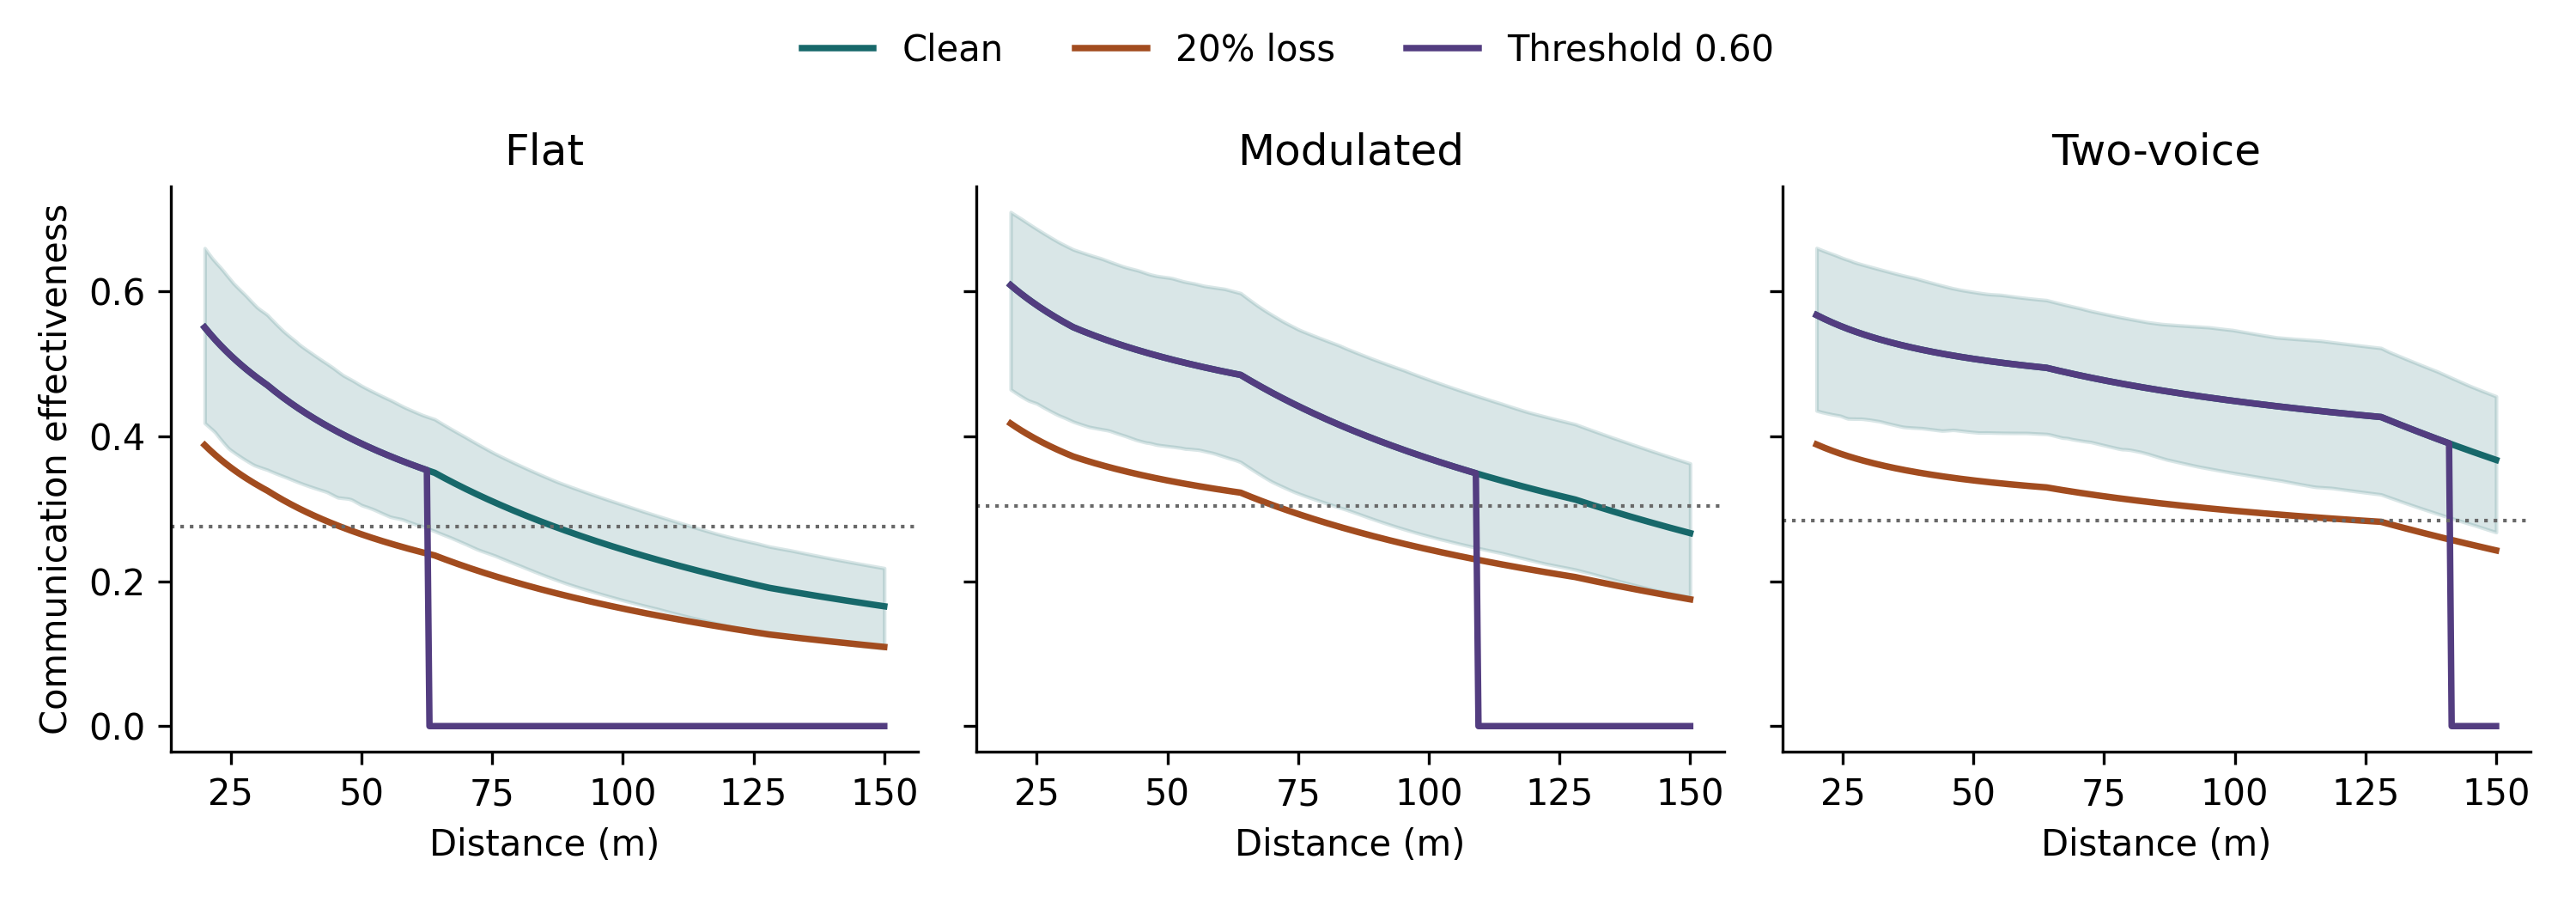
\includegraphics[width=\linewidth]{q4_scenarios.png}\\
{\small Figure C1. Archived call-specific clean references and alternative disturbance scenarios. Dotted lines mark the fixed clean cutoffs. Shading shows the clean conditional intervals.}
\end{minipage}\end{center}

\section{Analysis source}
The \evidence{README.md}{repository commands} reproduce the figures and tables from the supplied attachments. The noise simulation uses the three example WAVs. The video audit uses the original MP4 locally.

\subsection{Software}
The analysis used Python 3.10.11 with NumPy 2.2.6, pandas 2.3.3,
SciPy 1.15.3, scikit-learn 1.7.2, Matplotlib 3.10.8,
statsmodels 0.14.6, and XGBoost 3.2.0. The paper was built with
\texttt{pdflatex} (MiKTeX-pdfTeX 4.23, MiKTeX 25.12).
Poppler 24.04.0 was used to inspect the PDF.

\subsection{Core analysis and earlier sensitivity checks}
\lstinputlisting[caption={Core acoustic classification}]{../core_q1.py}
\lstinputlisting[caption={Core propagation validation}]{../core_q2.py}
\lstinputlisting[caption={Core playback masks and timing}]{../core_q3.py}
\lstinputlisting[caption={Core model integration and figures}]{../core_integration.py}
\lstinputlisting[caption={Reproduction entry point}]{../main.py}
\lstinputlisting[caption={Acoustic classification}]{../q1.py}
\lstinputlisting[caption={Acoustic propagation}]{../q2.py}
\lstinputlisting[caption={Playback behavior}]{../q3.py}
\lstinputlisting[caption={Communication effectiveness}]{../q4.py}
\lstinputlisting[caption={Representation and predictor ablations}]{../round2.py}
\lstinputlisting[caption={Final behavior comparisons and recording-group influence}]{../final_analysis.py}
\lstinputlisting[caption={Blocked peak-frequency associations}]{../creative_q1.py}
\lstinputlisting[caption={Pairwise mask model and ablation}]{../creative_q3.py}
\lstinputlisting[caption={Control background and fixed fidelity gate}]{../creative_gate.py}
\lstinputlisting[caption={Inverse loss scenarios}]{../creative_inverse.py}
\lstinputlisting[caption={Sparse mask and loss limit checks}]{../post_hoc.py}
\lstinputlisting[caption={Decision rules, crossed variance and trial allocation}]{../q4_decision.py}
\lstinputlisting[caption={Playback dependence and trial precision}]{../playback_dependence.py}
\lstinputlisting[caption={Matched distance, loss limits and weighted behaviors}]{../matched_sensitivity.py}

\lstinputlisting[caption={Attenuation fit and resampling checks}]{../physical_attenuation.py}
\lstinputlisting[caption={Acoustic feature transformations and recorded onset validation}]{../onset_analysis.py}
\lstinputlisting[caption={Noise power and individual responder bounds}]{../noise_scenarios.py}
\lstinputlisting[caption={Agreement across noise scenarios}]{../noise_agreement.py}
\lstinputlisting[caption={Strict playback and crossed resampling}]{../strict_playback.py}
\lstinputlisting[caption={False Bay sea-state sensitivity}]{../sea_state.py}
\lstinputlisting[caption={WAVERYS and assumed example deletion}]{../example_sensitivity.py}
\lstinputlisting[caption={Missing propagation comparisons}]{../missing_propagation.py}

\subsection{Playback behavior analyses}
\lstinputlisting[caption={Group size and response predictions}]{../group_size.py}
\lstinputlisting[caption={Vocal counts and contact scenarios}]{../vocal_counts.py}
\lstinputlisting[caption={Paired playback observation windows}]{../observation_window.py}
\lstinputlisting[caption={Head-raising duration, 30 s response and external noise}]{../playback_endpoints.py}
\lstinputlisting[caption={First replies and event order}]{../first_reply.py}
\lstinputlisting[caption={Response frequency and responder composition}]{../behavior_gap.py}
\lstinputlisting[caption={Observed first-playback response bounds}]{../q3_first_playback.py}
\lstinputlisting[caption={Playback carryover sensitivity}]{../q3_carryover.py}

\subsection{Integrated communication analyses}
\lstinputlisting[caption={Effectiveness and attainment over the supported annulus}]{../spatial_annulus.py}
\lstinputlisting[caption={Context mix and behavior priorities}]{../context_priority.py}
\lstinputlisting[caption={Discrete historical recovery scenarios}]{../recovery.py}
\lstinputlisting[caption={Continuous historical recovery certificate}]{../continuous_recovery.py}
\lstinputlisting[caption={Control subtraction and cutoff sensitivity}]{../control_subtraction.py}
\lstinputlisting[caption={Behavior model sensitivity}]{../behavior_ablation.py}
\lstinputlisting[caption={Intact-pair distance deletion}]{../distance_deletion.py}
\lstinputlisting[caption={Monte Carlo precision of distance-deletion decisions}]{../distance_deletion_mc.py}
\lstinputlisting[caption={Fisher planning for three Q4 margins}]{../q4_fisher.py}
\lstinputlisting[caption={Paired dependence in Q4 trial allocation}]{../q4_paired_planning.py}
\lstinputlisting[caption={Sensitivity to extrapolation drift after union deletion}]{../q4_extrapolation_drift.py}
\lstinputlisting[caption={Playback models and date-and-track validation for tail ablation}]{../q4_tail_models.py}
\lstinputlisting[caption={Paired Q4 tail ablation and drift comparisons}]{../q4_tail_ablation.py}
\lstinputlisting[caption={Tail validation by actual playback distance}]{../q4_tail_distance.py}
\lstinputlisting[caption={Candidate sets for held-out recording groups}]{../q1_candidate_sets.py}
\lstinputlisting[caption={Q2 rank changes along the envelope-weight path}]{../q2_envelope_rank.py}
\lstinputlisting[caption={Q2 spectral allocation sensitivity}]{../q2_spectral_allocation.py}
\lstinputlisting[caption={Q4 envelope-weight attainment intervals}]{../q4_envelope_attainment.py}
\lstinputlisting[caption={Direction of discordant playback responses}]{../q3_direction.py}
\lstinputlisting[caption={Q2 attenuation shape and weight ranks}]{../q2_shape_rank.py}
\lstinputlisting[caption={Q2 forward-distance validation}]{../q2_forward.py}
\lstinputlisting[caption={Q2 partial pooling of attenuation exponents}]{../q2_partial_pooling.py}
\lstinputlisting[caption={Q4 attenuation-shape propagation}]{../q4_shape_propagation.py}
\lstinputlisting[caption={Q4 acoustic and response-loss tradeoffs}]{../q4_net_loss.py}
\lstinputlisting[caption={Q4 consecutive-distance attainment}]{../q4_consecutive.py}
\lstinputlisting[caption={Q4 loss limits at target distances}]{../q4_target_loss.py}
\lstinputlisting[caption={Q4 acoustic and behavior draw rematching}]{../q4_draw_rematching.py}
\lstinputlisting[caption={Q4 consecutive-radius draw rematching}]{../q4_prefix_rematching.py}
\lstinputlisting[caption={Q4 local and matched uniform noise}]{../q4_matched_noise.py}
\lstinputlisting[caption={Q4 response sensitivity at 6 dB}]{../q4_response_sensitivity.py}
\lstinputlisting[caption={Q4 intermittent noise}]{../q4_intermittent_noise.py}
\lstinputlisting[caption={Q4 context-dependent exposure}]{../q4_context_exposure.py}
\lstinputlisting[caption={Q4 context Monte Carlo precision}]{../q4_context_mc.py}
\lstinputlisting[caption={Q4 independent full-fit precision follow-up}]{../q4_context_followup.py}
\lstinputlisting[caption={Q4 bounded-context behavioral noise sensitivity}]{../q4_context_lambda.py}
\lstinputlisting[caption={Matched-power noise simulation for the three example calls}]{../appendix5_noise.py}
\lstinputlisting[caption={Noise, participation and field-design figures}]{../core_paper_figures.py}
\subsection{Classification and monitoring sensitivity}
\lstinputlisting[caption={Class-prior decision rules}]{../q1_class_prior.py}
\lstinputlisting[caption={Recording-location sensitivity}]{../q1_location.py}
\lstinputlisting[caption={Propagation of classification errors into monitoring}]{../q1_q4_labels.py}
\lstinputlisting[caption={Cost-sensitive monitoring decisions}]{../q1_q4_cost.py}
\lstinputlisting[caption={Monitoring baselines without acoustic features}]{../q1_q4_prevalence.py}
\lstinputlisting[caption={Score-guided manual review}]{../q4_score_review.py}
\lstinputlisting[caption={Monitoring review budgets}]{../q4_review_budget.py}
\end{document}






